\section{Discussion}\label{sec:discussion}

First comprehensive analysis of Sgr A* including both resolved VLBI data and multiwavelength data.

Discussion organized according to physical parameters of the model.

\note{Avoid figures where possible.}

%==============================================================================
\subsection{MAD, SANE, and Self-Consistent Wind Feeding}

\note{Angelo to provide first draft}

There are clear differences between MAD and SANE models in VLBI data, as well as in the non-VLBI data.

Assessment of Ressler model.  Viable!

%==============================================================================
\subsection{Electron Distribution Function}

\note{Koushik to provide first draft}

Strong constraint on abundance of cold electrons from bremss.  A high density of cold electrons - which would be invisible in synchrotron - are ruled out.  This is in part because at $\Theta_e \equiv k T_e/(m_e c^2) \lesssim 1$, $j_\nu \propto \Theta_e^{-1/2}$ (emission in the x-ray band increases as temperature decreases).  In contrast, for $\Theta_e \gtrsim 1$ electron-electron bremsstrahlung becomes important and $j_\nu \propto \Theta_e^{+1/2}$.

Strong constraint on abundance of hot electrons from NIR.  In particular for

Strong constraint on $T_i/T_e$: models with ion temperature equal to electron temperature fail on several counts.

%==============================================================================
\subsection{Inclination}

\note{Michi to provide first draft}

Strong constraints on inclination from m-ring fitting.

%==============================================================================
\subsection{Position Angle}

Virtually no constraint on position angle [check m-ring fits]

%==============================================================================
\subsection{Black Hole Spin}

Still quite weak constraints on black hole spin.

%==============================================================================
\subsection{Accretion Rate and Outflow Power}

\note{Vedant to provide first draft of thermal section.}

We compute the outflow power in a fashion similar to that in \citet{M87PaperV},

\begin{equation}
    P_{out} = \int_{funnel}d\theta\frac{1}{\Delta t}\int dtd\phi\sqrt{-g}\big(-T^{r}_{t}-\rho u^{r}\big),
\end{equation}

evaluated at $r=100GM/c^{2}$, where $funnel\Rightarrow(\theta<1)\cup(\theta>\pi-1)$. We average the quantity in time $\Delta t$, where $\Delta t$ is the time interval we have considered for our analysis. We also consider only those regions where there is steady outflow, ie. the quantity in the parentheses is positive.

\begin{figure*}
\centering
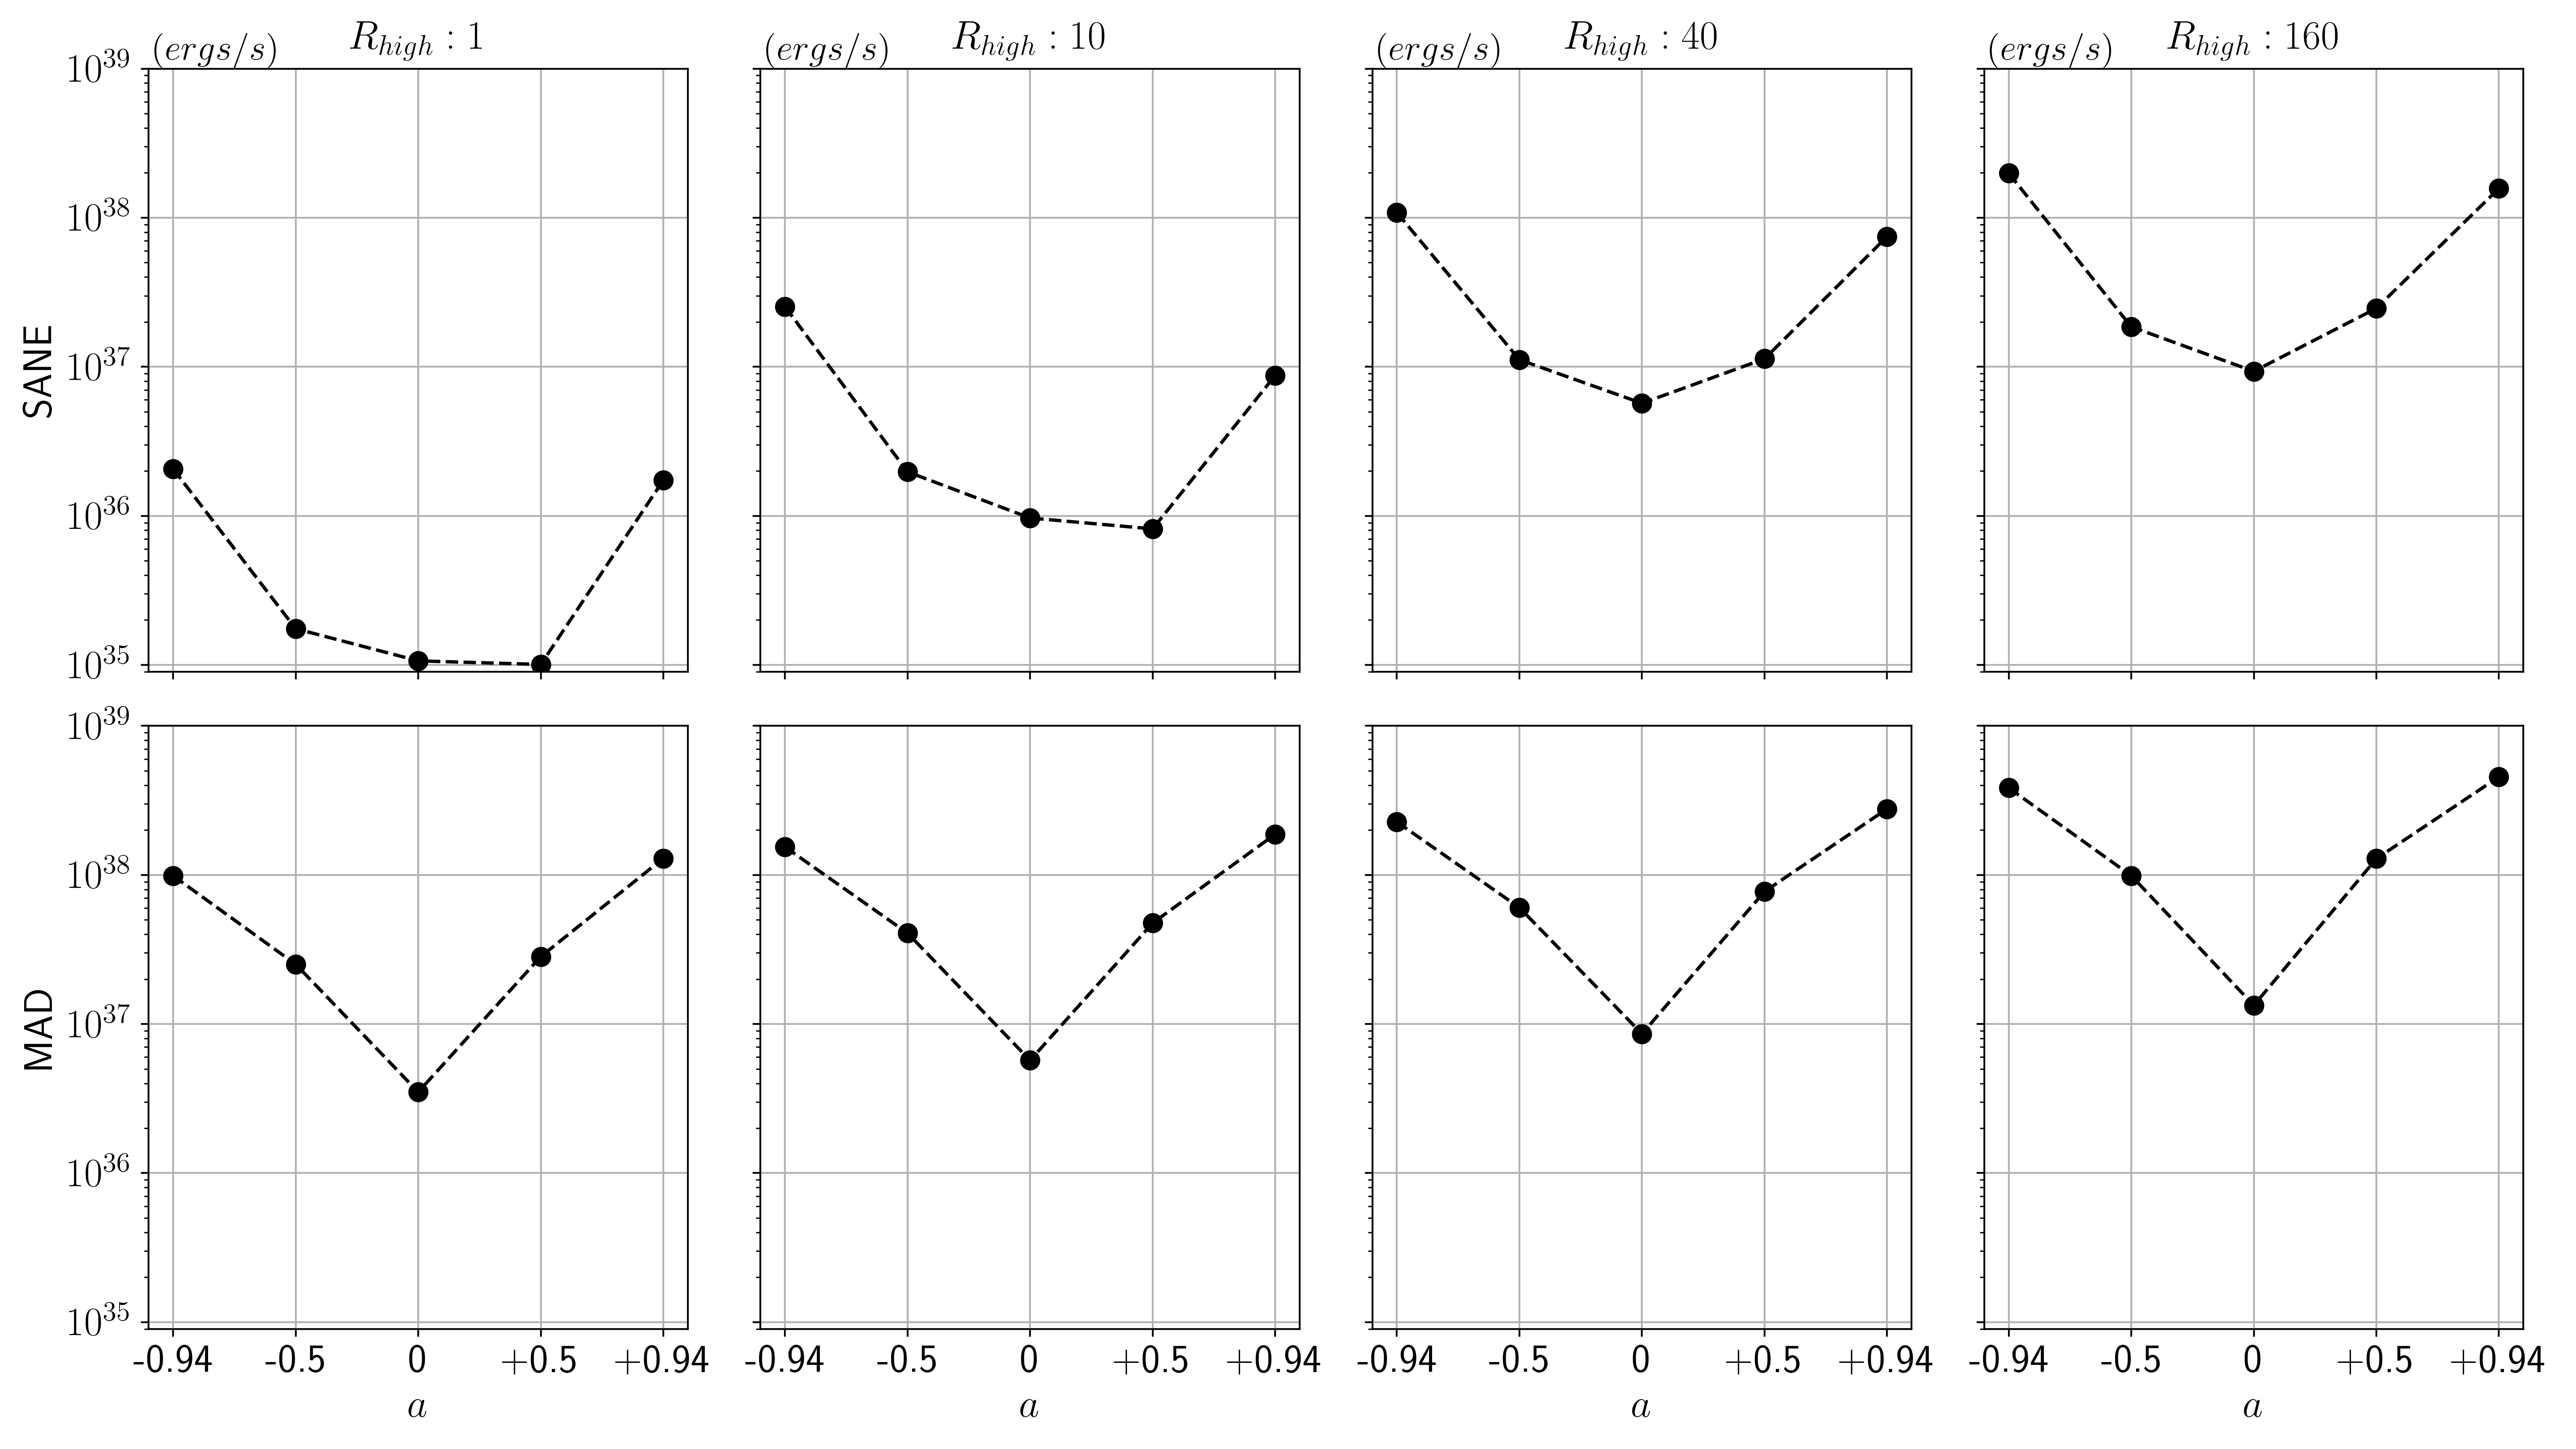
\includegraphics[width=0.95\textwidth]{figures/illinoisv3_total_output_power.png}
\caption{Outflow power for Illinois-Thermal models}
\label{fig:outflow_illinois_thermal}
\end{figure*}

\begin{figure*}
\centering
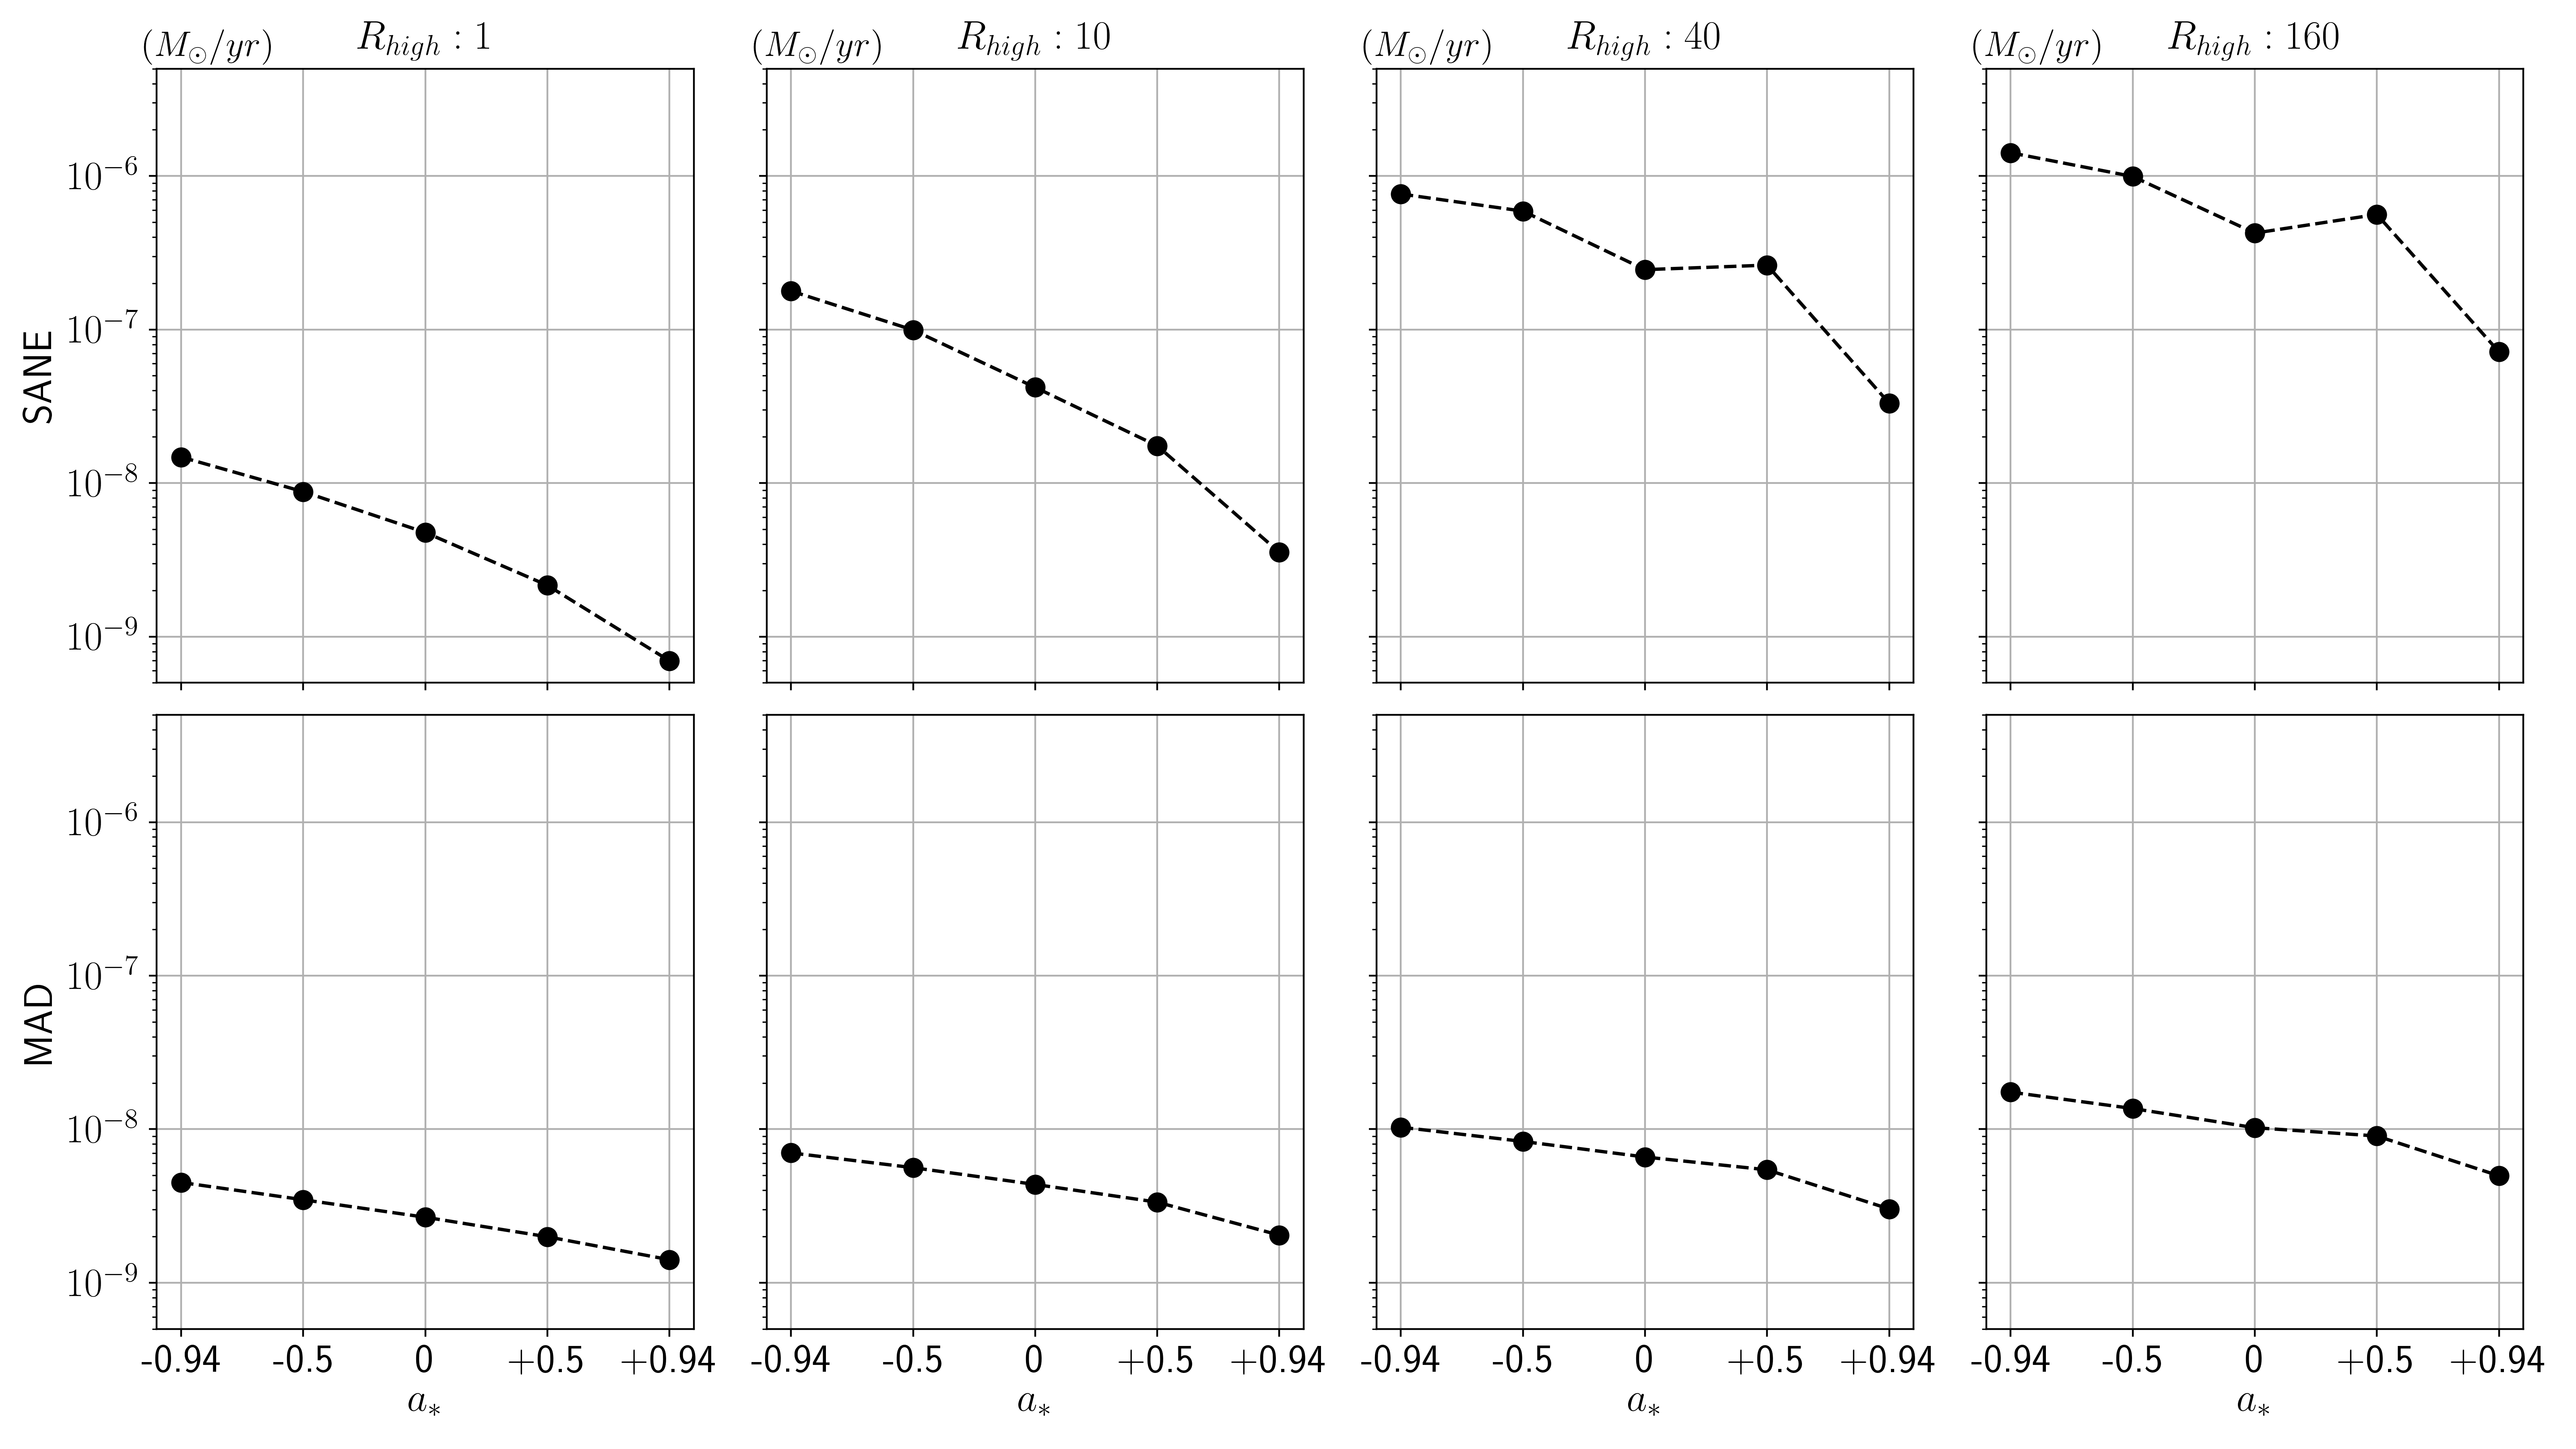
\includegraphics[width=0.95\textwidth]{figures/illinoisv3_average_munit.png}
\caption{Accretion rate for Illinois-Thermal models}
\label{fig:accretion_illinois_thermal}
\end{figure*}

Figure showing accretion rate.

Accretion rate is consistent with earlier analyses.

Models at the highest accretion rate are ruled out by overproduction of x-ray emission.  If our models were in equilibrium over a larger range in radius, bremss from larger radius might increase the x-ray flux and rule out more models.

Figure showing outflow power.

Jet power is surprisingly large.  Where does the power come out in the galactic center?

Dependence on distribution function.

\note{Koushik, Alejandro, Razi}

%==============================================================================
%\subsection{Analytical Accretion Models
%  [Pu, Anantua, Jeter]}
%\label{sec:anamodels}

\subsection{Positrons}

\ckc{Review panel suggested not to include RIAF model.  Please repurpose this section to discuss positrons.  Avoid figures when possible.}

\cite{Broderick2005} devised a canonical model of Sgr A* as a  radiatively inefficient accretion flow (RIAF). Semi-analytic RIAF models implementing  this using the general relativistic ray tracer GRTRANS \citep{2016MNRAS.462..115D} can be found in  \cite{Emami2021}, where  positrons are included using emission modeling motivated in  \cite{Anantua:2019bna}. The Fig. \ref{fig:EmamiRIAF} model from \cite{Emami2021}  shows Stokes maps and polarized spectra of a \cite{Broderick2005} RIAF with plasma $\beta=10$ and 1$\%$ of the emitting particles nonthermal electrons. The near-extremal ($a/M=0.998$) model shown exhibits Doppler boosting asymmetry in a crescent-shaped intensity pattern with a spiral global electric vector polarization angle (EVPA) pattern and polarization preferentially distributed within this region.

The addition of small non-thermal populations of positrons \citep{Anantua:2019bna,Emami2021} tends to: increase overall intensity in jet regions for fixed electron number density; modify the low-frequency spectral slope; cancel the observed intrinsic circular polarization and enhance circular polarization due to Faraday conversion. The last of these positron effects is particularly apparent when comparing declining tails of x-ray spectra of positron-rich versus positron-poor sources, as seen in Fig. \ref{fig:EmamiRIAFSpectra}.

%\begin{figure}%[H]
%   \plotone{RIAFSgrAPlaneTscl1Pt5e11beta1Pt0e01fpos0Pt0fNTH1Pt0e-02copy.png}
%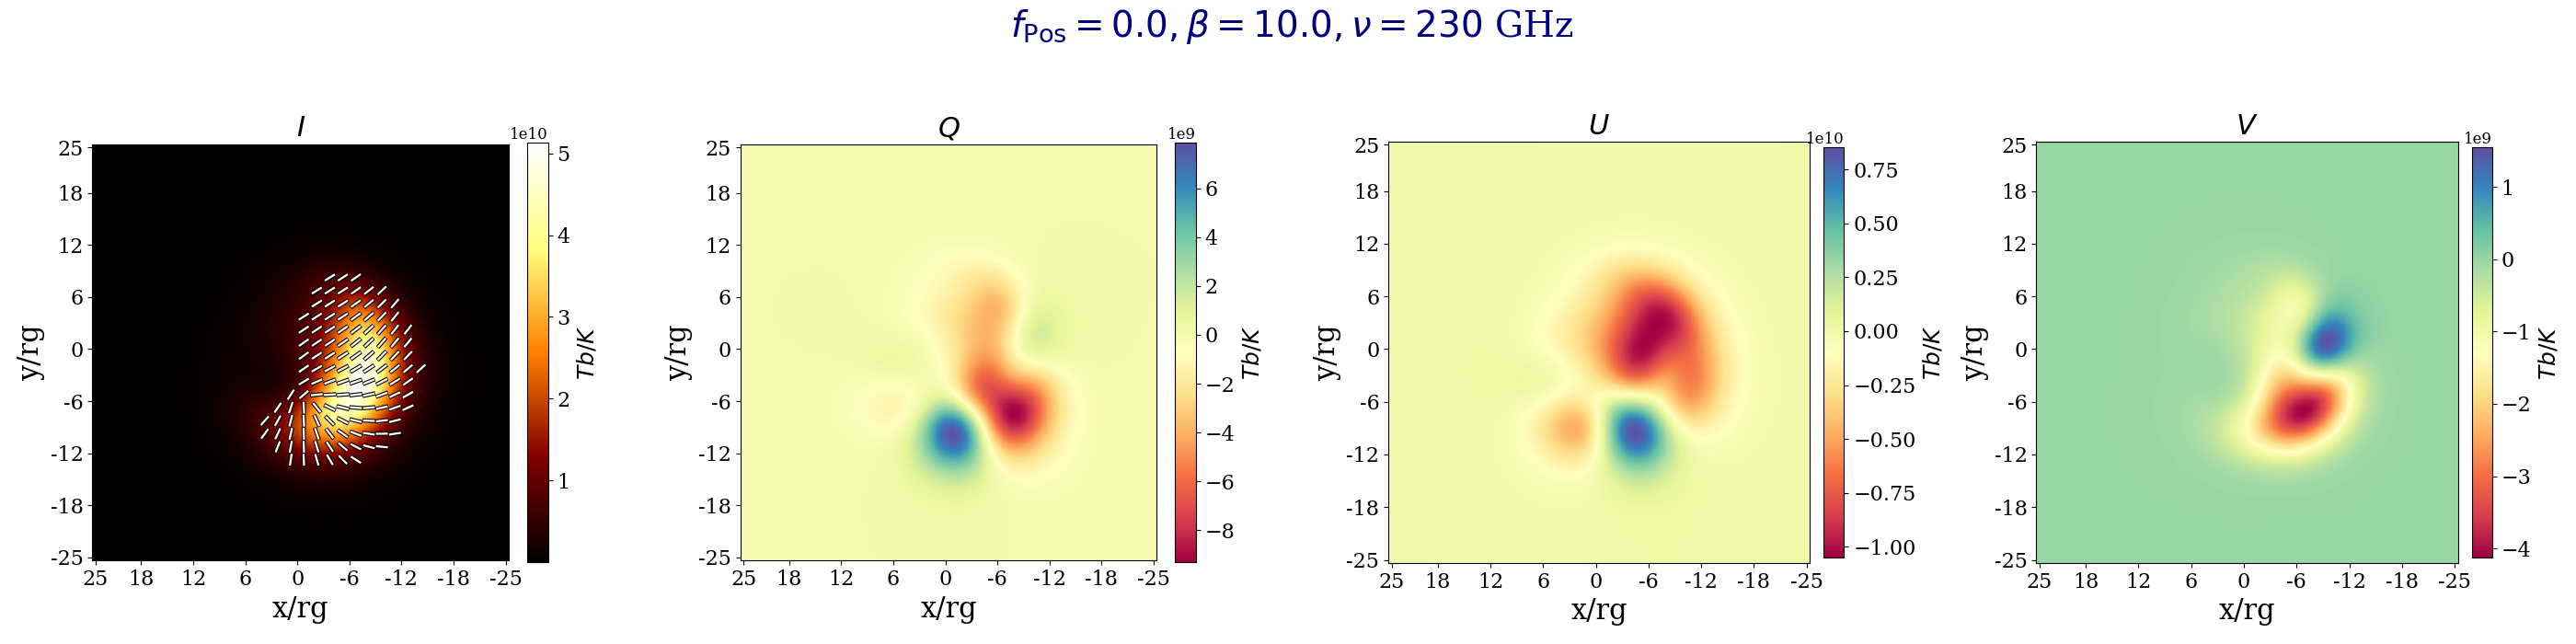
\includegraphics[width=.5\textwidth,height=27mm%,trim=0 380 0 200,clip
%]{RIAFSgrAPlaneTscl1Pt5e11beta1Pt0e01fpos0Pt0fNTH1Pt0e-02copy}
%  \caption{Polarization maps of Stokes parameters $I$, $Q$, $U$ and $V$ at 230 GHz for a \cite{Broderick2005} RIAF with $\beta=10$.}
%  \label{fig:EmamiRIAF}
%\end{figure}

%\begin{figure}%[H]
%\begin{figure*}%[H]
%   \plotone{RIAFSgrAPlaneTscl1Pt5e11beta1Pt0e01fpos0Pt0fNTH1Pt0e-02copy.png}
%  \includegraphics[width=.4\textwidth%width=.55\textwidth,height=25mm%,trim=0 380 0 200,clip
%]{PositronModelEtAl2021RIAFPolSpectra%PolSpectscl1Pt5e11Beta1Pt0e1nth1Pt0em2fpos0Pt0
%}
%  \caption{Polarized SEDs for the Sgr A* RIAF model with  $\beta\in\{10^{-2},10^{0},10^{1}\}$, $f_\mathrm{pos}\in\{0.0,0.5,1.0\}$. The Top Panel shows the Stokes $I$ spectrum, while the Middle Panel shows the SED in linear polarization and the Bottom Panel shows the same for circular polarization.}
%  \label{fig:EmamiRIAFSpectra}
%\end{figure*}
%\end{figure}

%MOVED from Sect. 3.1 to Sect. 3.0
% \textcolor{red}{RJA: Include a summary of analytic/semi-analytic models and Sgr A* simulations in the Literature} Analytic disk $\alpha$-model for angular momentum transport \cite{Shakura1973}. Semi-analytic model motivated in \cite{Yuan2003} and expanded in \cite{Broderick2011}. GRMHD Simulation with hotspots reproducing Sgr A* flares \cite{Ripperda2020}.

\note{to be discussed: how much we would like to discuss polarization emission?}\textcolor{red}{RJA: We should mention the M87 Polarization Collaboration papers \cite{EHTCPaperVII}, including a comparison of whether Sgr A* is similar enough (e.g., MAD with vertical fields Faraday depolarized on much of the accretion flow) to have an azimuthally spiral EVPA pattern. Figures in  \citep{Emami2021} have similar morphology}.

\hyp{to-do :  adding historical RIAF fitting result to proto-EHT observations; how recent  GRMHD simulation and subsequent GRRT post-processing suggest other key parameters onto the Broderick 2005 RIAF model; jet componenet? cross referencing MCFE RIAF analysis product?} A proto-EHT array described in \cite{Doeleman2008} estimated the Sgr A* emitting region profile as a circular Gaussian with intrinsic size $37^{+16}_{-10}\ \mu$as.

% EHT flux vs. baseline observations constrain the emitting region intrinsic size to 37 microarcseconds for a circular Gaussian emission profile

More recent measurements of closure phases of a few degrees \cite{Fish2016} suggest an asymmetric ring-like profile, with major axis 56 microarcseconds

%==============================================================================
\subsection{Caveats and Limitations}

\br{The mean free path to collisions for particles is typically larger than or comparable to the system size for \sgra, rendering the plasma collisionless. The GRMHD models employed in this work, describe a collisional system, whereas a first-principles modeling of the collisionless plasma requires a fully kinetic treatment. General relativistic (radiative) kinetic simulations, e.g., \cite{2018A&A...616A.184L,2018ApJ...863L..31C,2019PhRvL.122c5101P,2020PhRvL.124n5101C,2020ApJ...895..121C,2020ApJ...902...80K,2021A&A...650A.163C,2021PhRvL.127e5101B}, are crucial for probing non-thermal effects in the observed radiation and the impact of the electron temperature in collisionless plasma in the accretion disk and jet. Some aspects of collisionless plasma dynamics have been incorporated in non-ideal GRMHD models for black hole accretion, e.g.,  \cite{2014MNRAS.440L..41B,2015ApJ...810..162C,2016MNRAS.456.1332F,2017ApJ...837...92C,2017MNRAS.470.2240F,2018ApJ...859...28Q,2019ApJS..244...10R,2019ApJ...882....2V,2020ApJ...900..100R,2021arXiv211103689N,2021arXiv211105752M}. Even in GRMHD, it is computationally challenging to resolve heating processes in a converged manner. It is currently not yet feasible to resolve dissipation at the smallest scales of the turbulent cascade or the interplay between turbulence and reconnection at a similar level as in local box simulations \citep{2012ApJ...755...50R,2013ApJ...773..118H,2015PhRvL.114f1101H,2016PhRvL.117w5101K,2017PhRvL.118e5103Z,2018PhRvL.121y5101C,2018ApJ...859..149I,2019PhRvL.122e5101Z,2021ApJ...921...87N,2021arXiv211108188C}. Some efforts have recently been made with high-resolution global GRMHD simulations to capture heating through magnetic reconnection in the largest current sheets in the system \citep{2020MNRAS.495.1549N,2020ApJ...900..100R,2021MNRAS.508.1241C,2021arXiv210915115R,2021arXiv211103689N}. However, \citep{2019ApJS..243...26P} and \citet[in prep]{Olivares_et_al} show that the global accretion dynamics (mass accretion rate, magnetic flux on the horizon, and MRI quality factor) are resolved in our simulations.}

%==============================================================================
\subsection{Future Constraints}

integrated polarization,

resolved polarization

fits to more sophisticated models such as RIAF analytic models,

closure phase variability
